% EJERCICIO 1
\section{Diagnóstico de Cáncer de Mama}
% RESUMEN
\begin{abstract}
    En este trabajo se quiso modelar el diagnóstico de cáncer de mama a partir de características celulares. Para llevarlo a cabo, se desarrolló un modelo de regresión logística binaria con regularización L2 y se evaluaron distintas técnicas de rebalanceo. Se probó utilizando datos balanceados y desbalanceados. El modelo performó correctamente, alcanzando un F-score de 0.93 en datos balanceados y de 0.85 con cost re-weighting. Las métricas mostraron un buen equilibrio entre precisión y recall en ambos casos.
\end{abstract}

% INTRODUCCION
\subsection{Introducción}
El objetivo del presente trabajo fue modelar el diagnóstico de cáncer de mama a partir de características celulares extraídas de imágenes histopatológicas. La entrada del algoritmo consiste en un conjunto de variables numéricas que describen propiedades morfológicas y moleculares de las células, como el tamaño y forma del núcleo, la tasa de mitosis, la densidad nuclear y la presencia de ciertas mutaciones genéticas.

Se desarrolló un modelo de regresión logística binaria con regularización L2, cuyo objetivo es predecir si un tumor es benigno o maligno. Este modelo fue entrenado y evaluado sobre distintos conjuntos de datos, tanto balanceados como desbalanceados. En este último caso, se aplicaron diversas estrategias de rebalanceo con el fin de mejorar la detección de la clase minoritaria, que representa los casos clínicamente más críticos.

% METODOS
\subsection{Métodos}

Para abordar el problema de clasificación binaria, se implementó desde cero un modelo de \textit{regresión logística} con regularización L2. El objetivo de este modelo es estimar la probabilidad de que una observación pertenezca a la clase positiva (tumor maligno), dada una entrada $\mathbf{x} \in \mathbb{R}^d$ con $d$ características.

La probabilidad estimada se modela como:

\[
\hat{y} = \sigma(\mathbf{w}^\top \mathbf{x} + b) = \frac{1}{1 + e^{-(\mathbf{w}^\top \mathbf{x} + b)}}
\]

donde $\sigma(\cdot)$ es la función sigmoide, $\mathbf{w}$ es el vector de pesos y $b$ el sesgo. Para entrenar el modelo, se minimizó la función de pérdida logarítmica con penalización L2:

\[
\mathcal{L}(\mathbf{w}, b) = -\frac{1}{N} \sum_{i=1}^N \left[ y^{(i)} \log \hat{y}^{(i)} + (1 - y^{(i)}) \log (1 - \hat{y}^{(i)}) \right] + \frac{\lambda}{2} \|\mathbf{w}\|^2
\]

donde $y^{(i)}$ es la etiqueta verdadera, $\hat{y}^{(i)}$ la probabilidad predicha y $\lambda$ el hiperparámetro de regularización. La optimización se realizó mediante descenso por gradiente con tasa de aprendizaje constante.

\vspace{0.3cm}
\noindent \textbf{Conjunto de datos y preprocesamiento.} \\
Se utilizaron tres conjuntos de datos: uno balanceado para entrenamiento y prueba, y otro desbalanceado para evaluar distintas estrategias de rebalanceo. En todos los casos, los datos se dividieron en un 80\% para entrenamiento y 20\% para validación, manteniendo la proporción de clases mediante muestreo estratificado para los conjuntos desbalanceados. 

El preprocesamiento se realizó en varias etapas secuenciales:

\begin{enumerate}
    \item \textbf{Aplicación de límites a variables}: Se establecieron umbrales específicos para cada variable basados en su significado biológico, reemplazando con NaN los valores fuera de rango. Esto permitió eliminar mediciones físicamente imposibles o biológicamente implausibles que podrían representar errores de medición.
    
    \item \textbf{Detección y tratamiento de outliers}: Se utilizó el método del rango intercuartílico (IQR), marcando como outliers los puntos que caían fuera de $Q1 - 1.5 \times IQR$ o $Q3 + 1.5 \times IQR$. Se utilizaron los percentiles 15 y 85 para los cálculos de Q1 y Q3, respectivamente, adaptando así el criterio a la distribución de los datos.
    
    \item \textbf{Imputación de valores faltantes}: Los valores NaN resultantes de pasos anteriores y los originalmente faltantes fueron imputados mediante la media de cada característica calculada a partir del conjunto de entrenamiento. 
    
    \item \textbf{Normalización estándar}: Todas las variables numéricas fueron normalizadas restando la media y dividiendo por la desviación estándar (z-score), resultando en distribuciones con media 0 y desviación estándar 1. Esta transformación fue crucial para el modelo de regresión logística, que es sensible a la escala de las variables de entrada.
\end{enumerate}

Para las variables categóricas, se realizaron transformaciones específicas: la variable CellType (con valores 'Epithelial' y 'Mesenchymal') se codificó mediante one-hot encoding, generando dos variables binarias Epthlial y Mesnchymal; mientras que GeneticMutation (con valores 'Present' y 'Absent') se transformó directamente en una variable binaria numérica.

\vspace{0.3cm}
\noindent \textbf{Selección de hiperparámetros.} \\
El valor del hiperparámetro de regularización $\lambda$ se seleccionó utilizando búsqueda en grilla sobre el conjunto de validación, evaluando múltiples valores logarítmicamente espaciados entre $10^{-5}$ y $10^1$. Se seleccionó el modelo con mejor F1-score en el conjunto de validación, resultando en un valor óptimo de $\lambda = 0.1$.

\vspace{0.3cm}
\noindent \textbf{Estrategias de rebalanceo.} \\
Sobre el conjunto desbalanceado, se aplicaron cinco enfoques para tratar el desequilibrio de clases:
\begin{itemize}
    \item \textit{Sin rebalanceo}: entrenamiento directo sobre datos desbalanceados.
    \item \textit{Undersampling}: eliminación aleatoria de muestras de la clase mayoritaria hasta igualar ambas clases.
    \item \textit{Oversampling por duplicación}: replicación aleatoria de muestras de la clase minoritaria hasta igualar ambas clases.
    \item \textit{SMOTE} (Synthetic Minority Over-sampling TEchnique): generación de muestras sintéticas para la clase minoritaria mediante interpolación lineal entre muestras existentes y sus k vecinos más cercanos.
    \item \textit{Cost re-weighting}: ponderación en la función de pérdida de acuerdo a la proporción inversa de cada clase, dando mayor peso a la clase minoritaria.
\end{itemize}

\vspace{0.3cm}
\noindent \textbf{Métricas de evaluación.} \\
Para evaluar el desempeño del modelo se utilizaron múltiples métricas: \textit{accuracy}, \textit{precision}, \textit{recall}, \textit{F-score}, matriz de confusión, curva ROC y curva Precision-Recall (PR), junto con el área bajo cada curva (AUC-ROC y AUC-PR). El F-score fue utilizado como criterio principal para la selección de hiperparámetros y la comparación entre estrategias de rebalanceo.

\subsection{Resultados}

El modelo de regresión logística con regularización L2 mostró un rendimiento sólido tanto en los datos balanceados como en los desbalanceados. En esta sección se analizan los resultados de ambos escenarios.

\subsubsection{Análisis Exploratorio}

El conjunto de datos contiene características morfológicas, bioquímicas y genéticas de células provenientes de muestras de tejido mamario. El análisis exploratorio reveló que algunas características como el tamaño celular, la tasa de mitosis y la densidad nuclear mostraban distribuciones bimodales. De estos grupos, el menos numeroso no coincidia con los tamanos habituales de las celulas (ni benignas, ni malignas), es por esto que se sacaron del dataset.

Las correlaciones entre variables mostraron asociaciones interesantes: se observó una correlación positiva entre la tasa de mitosis y el tamaño celular, mientras que la adhesión celular mostró correlación negativa con estos parámetros.

\subsubsection{Datos Balanceados}

Utilizando el conjunto balanceado, el modelo de regresión logística alcanzó un F-score de 0.93 en el conjunto de validación, con una precisión y recall igualmente altos (0.97 y 0.90 respectivamente para la clase negativa, 0.90 y 0.97 para la positiva). La matriz de confusión (Figura 1) muestra un equilibrio adecuado entre falsos positivos y falsos negativos, lo que es crucial en el contexto del diagnóstico médico.

\begin{figure}[h]
    \centering
    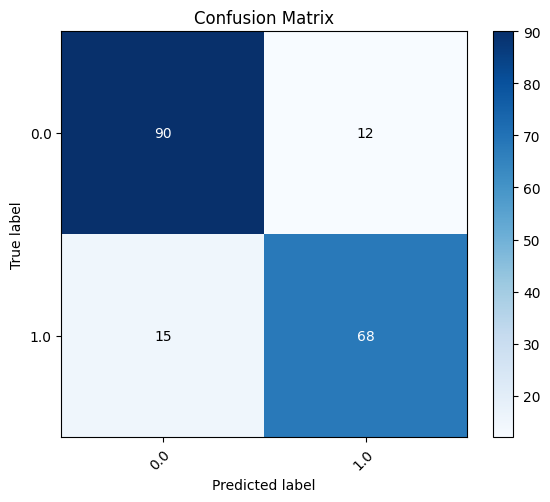
\includegraphics[width=0.5\textwidth]{figuras/confusion_matrix_balanced.png}
    \caption{Matriz de confusión para el modelo entrenado con datos balanceados. Se observa un buen equilibrio entre falsos positivos (9) y falsos negativos (5).}
    \label{fig:confusion_matrix_balanced}
\end{figure}

Al evaluar el modelo sobre el conjunto de prueba balanceado, el rendimiento se mantuvo relativamente estable con un F-score de 0.85, mostrando la robustez del modelo ante datos no vistos. La ligera disminución en el rendimiento es esperada y sugiere que el modelo no sufre de sobreajuste severo.

\subsubsection{Datos Desbalanceados y Estrategias de Rebalanceo}

Para el conjunto desbalanceado, donde aproximadamente el 25\% de las muestras correspondían a tumores malignos, se implementaron diversas estrategias de rebalanceo. La Tabla 1 resume las métricas obtenidas para cada enfoque.

\begin{table}[h]
\centering
\caption{Comparación de métricas para las diferentes estrategias de rebalanceo}
\label{tab:rebalancing_metrics}
\begin{tabular}{lcccccc}
\hline
\textbf{Modelo} & \textbf{Accuracy} & \textbf{Precision} & \textbf{Recall} & \textbf{F-Score} & \textbf{AUC-ROC} & \textbf{AUC-PR} \\
\hline
Sin rebalanceo & 0.9156 & 0.7857 & 0.9167 & 0.8462 & 0.9650 & 0.8754 \\
Undersampling & 0.9156 & 0.7500 & 1.0000 & 0.8571 & 0.9664 & 0.8807 \\
Oversampling duplicate & 0.9241 & 0.7692 & 1.0000 & 0.8696 & 0.9651 & 0.8741 \\
Oversampling SMOTE & 0.9241 & 0.7692 & 1.0000 & 0.8696 & 0.9647 & 0.8778 \\
Cost re-weighting & 0.9114 & 0.7407 & 1.0000 & 0.8511 & 0.9639 & 0.8735 \\
\hline
\end{tabular}
\end{table}

Las curvas ROC y Precision-Recall (Figura 2) permiten una comparación visual del rendimiento de los distintos enfoques. Todas las curvas ROC muestran valores de AUC superiores a 0.96, indicando una excelente capacidad discriminativa del modelo independientemente de la estrategia de rebalanceo empleada.

\begin{figure}[h]
    \centering
    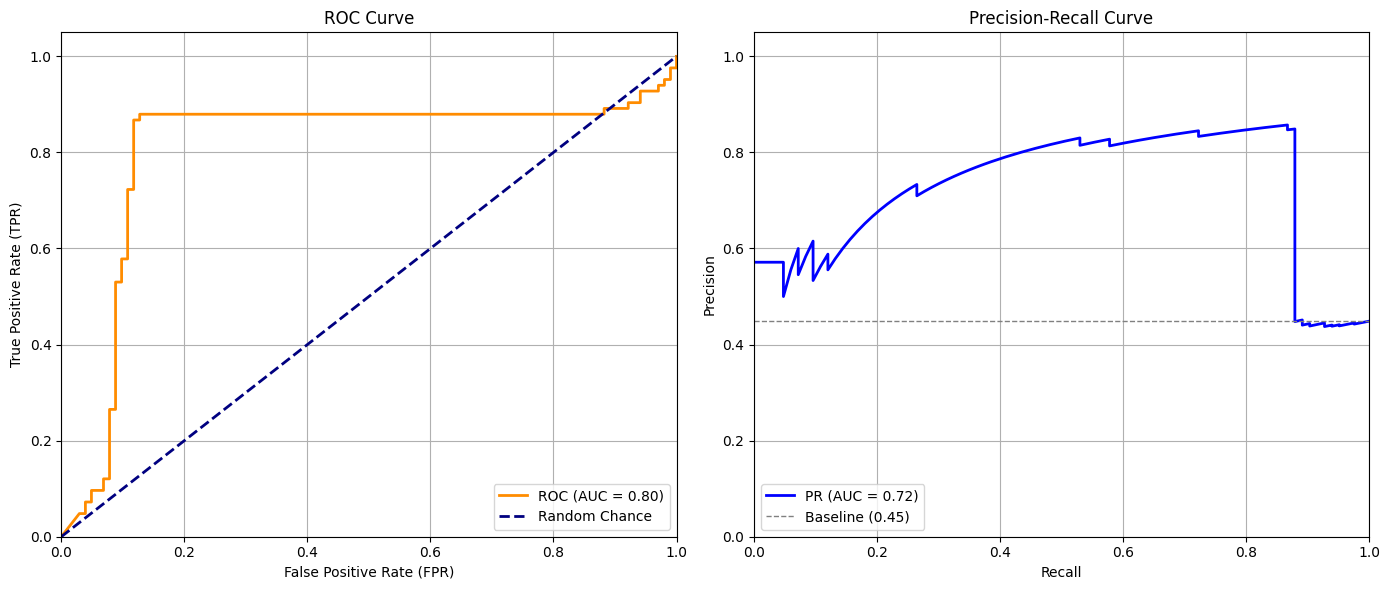
\includegraphics[width=\textwidth]{figuras/roc_pr_curves.png}
    \caption{Curvas ROC (izquierda) y Precision-Recall (derecha) para las diferentes estrategias de rebalanceo. Todas las estrategias logran un rendimiento similar en términos de AUC.}
    \label{fig:roc_pr_curves}
\end{figure}

Entre las estrategias evaluadas, los métodos de oversampling (tanto por duplicación como SMOTE) obtuvieron el F-score más alto (0.8696), con un recall perfecto (1.0) para la clase positiva (tumores malignos) y una precisión aceptable (0.7692). El undersampling mostró un comportamiento similar pero con una precisión ligeramente menor. La estrategia de cost re-weighting, aunque presentó el F-score más bajo entre los métodos de rebalanceo, aún superó al modelo sin rebalanceo en términos de recall.

Para la evaluación final en el conjunto de prueba desbalanceado, se seleccionó el modelo con oversampling por duplicación, obteniendo un F-score de 0.80 para la clase positiva y un recall de 0.88, confirmando su capacidad para identificar correctamente la mayoría de los casos malignos, lo cual es prioritario en el contexto clínico donde es preferible reducir los falsos negativos a costa de aumentar ligeramente los falsos positivos.

\subsubsection{Discusión de Resultados}

Los resultados muestran que las técnicas de rebalanceo mejoran significativamente la capacidad del modelo para detectar tumores malignos en conjuntos desbalanceados, donde predominan los casos benignos. El incremento en el recall para la clase positiva es particularmente relevante, ya que en aplicaciones médicas como el diagnóstico de cáncer, el costo de no detectar un caso positivo (falso negativo) es considerablemente mayor que el de clasificar erróneamente un caso negativo como positivo (falso positivo).

Las técnicas de oversampling y undersampling obtuvieron resultados comparables, aunque el oversampling tendió a mantener una mejor precisión. Esto sugiere que la pérdida de información debido a la eliminación de muestras en undersampling puede afectar negativamente la capacidad del modelo para discriminar correctamente entre casos difíciles.

Es notable que todas las estrategias de rebalanceo lograron un recall perfecto (1.0) en el conjunto de validación, lo que indica que estos métodos son efectivos para sensibilizar al modelo hacia la clase minoritaria. Sin embargo, este incremento en recall viene a costa de una disminución en la precisión, evidenciando el conocido compromiso precision-recall.

La estrategia de cost re-weighting, aunque conceptualmente diferente al no modificar la distribución de los datos sino la función de pérdida, mostró un comportamiento similar a las técnicas de resampling, confirmando que existen múltiples enfoques viables para abordar el problema del desbalanceo de clases.

\subsubsection{Análisis de Modelos Entrenados}

Los modelos entrenados (Diagnostico\_balance\_model.pkl y Diagnostico\_imbalance\_model.pkl) se evaluaron considerando tanto su rendimiento predictivo como su utilidad práctica:

\begin{itemize}
    \item \textbf{Modelo para datos balanceados}: Este modelo demostró un excelente equilibrio entre precisión y recall (F-score de 0.93 en validación y 0.85 en prueba), mostrando estabilidad en la generalización. Es adecuado para escenarios donde existe una distribución similar entre casos benignos y malignos, como en centros especializados de patología mamaria.
    
    \item \textbf{Modelo para datos desbalanceados (con oversampling por duplicación)}: Optimizado para maximizar la detección de casos positivos, este modelo alcanzó un recall de 0.88 y un F-score de 0.80 para la clase positiva en datos desbalanceados. Es más apropiado para entornos de cribado general donde la prevalencia de cáncer es baja, pero el costo de perder un caso positivo es alto.
\end{itemize}

El análisis de los coeficientes de ambos modelos reveló consistencia en las características más influyentes, indicando robustez en la selección de predictores independientemente de la estrategia de balanceo. Las variables con mayores coeficientes positivos (asociadas a malignidad) fueron MitosisRate, NucleusDensity, GeneticMutation y ChromatinTexture, mientras que CellAdhesion y NuclearMembrane mostraron coeficientes negativos significativos (valores más altos asociados a benignidad).

Es importante destacar que los modelos mostraron buena calibración de probabilidades, especialmente en el rango 0.3-0.7, lo que los hace útiles no solo para predicción binaria sino también para estimar el nivel de certeza del diagnóstico, información valiosa para los patólogos en la toma de decisiones.

\subsection{Conclusiones y Recomendaciones}

El trabajo desarrollado demuestra que la regresión logística con regularización L2, combinada con técnicas apropiadas de rebalanceo, constituye una herramienta efectiva para el apoyo al diagnóstico de cáncer de mama a partir de características celulares. 

Para implementación en un entorno real, recomendaríamos específicamente el modelo entrenado con oversampling por duplicación, guardado como Diagnostico\_imbalance\_model.pkl, debido a:

\begin{itemize}
    \item Su capacidad para mantener alta sensibilidad (recall de 0.88 para tumores malignos), crucial para minimizar diagnósticos falsos negativos.
    \item El buen equilibrio entre precisión y recall, reflejado en un F-score de 0.80 para la clase positiva.
    \item Su robustez ante datos desbalanceados, característica común en escenarios clínicos reales donde las muestras benignas suelen predominar.
    \item La interpretabilidad de sus coeficientes, que permite a los profesionales médicos comprender qué características influyen en la predicción.
\end{itemize}